\documentclass[letterpaper,11pt]{scrreprt}
\usepackage[american]{babel}
\usepackage[latin1]{inputenc}
\usepackage[T1]{fontenc}
\usepackage[top=1in,bottom=1in,left=1in,right=1in]{geometry}
\usepackage{lmodern}

\usepackage[sumlimits]{amsmath}
\usepackage{amssymb}
\usepackage{relsize}
\usepackage[hyperref]{ntheorem}
\usepackage[
	bookmarks,
	colorlinks=false,
	breaklinks=true,
	linkcolor=blue,
	citecolor=blue,
	pagebackref=false,
	pdftitle={MADlib Design Document},
	pdfauthor={Predictive Analytics Team, Pivotal Inc.},
	pdfsubject={},
	pdfkeywords={}
]{hyperref}
\usepackage{csquotes}                  % Strongly recommended for biblatex
\usepackage[
	backend=bibtex,
	maxnames=2,
	maxbibnames=20,
	firstinits=true
]{biblatex}
\usepackage{scrpage2}                  % Headers and footers
\usepackage{scrhack}
\usepackage{color}                     % Colors, possibly only for \todo
\usepackage{enumitem}                  % enumerate environment
\usepackage{ctable}
\usepackage{tabularx}
\usepackage{xspace}                    % Correct spaces after \newcommand definitions
\usepackage[noend]{algpseudocode}      % algorithm environment
\usepackage{listings}                  % Code snippets
\usepackage{bbding}

% BEGIN Doc Layout
	\allowdisplaybreaks[3]

	\pagestyle{scrheadings}
	\automark[chapter]{section}

	\setkomafont{disposition}{\normalcolor\bfseries}
	\setkomafont{descriptionlabel}{\bfseries}
	\setkomafont{captionlabel}{\usekomafont{disposition}}

	\setlength{\arrayrulewidth}{.5pt}
	\numberwithin{equation}{section}
	\renewcommand{\theenumi}{\roman{enumi}}
	\renewcommand{\labelenumi}{\theenumi)}

	\newcommand{\otoprule}{\midrule[\heavyrulewidth]}

	\setcounter{secnumdepth}{3}

	\makeatletter
	% Algorithms are expected to have an optional argument of form
	% FunctionName$(ArgumentList)$, e.g., DiscreteSample$(A, w)$
	\def\internal@funcName#1$(#2)${#1}
	\newcommand\funcName[1]{\internal@funcName #1}
	\newtheoremstyle{algorithm}
		{\item[\rlap{\vbox{\hbox{\hskip\labelsep \theorem@headerfont
			##1\ ##2\theorem@separator}\hbox{\strut}}}]}%
		{\item[\rlap{\vbox{\hbox{\hskip\labelsep {\theorem@headerfont
			##1}\ \normalfont\texttt{##3}{\theorem@headerfont\theorem@separator}}\hbox{\strut}}}]%
			\def\@currentlabel{\texttt{\funcName{##3}}}}
	\makeatother

	\makeatletter
	% Also display JSTOR in small caps
	% http://sourceforge.net/tracker/index.php?func=detail&aid=3152938&group_id=244752&atid=1126006
	\DeclareFieldFormat{eprint:arxiv}{%
	  \textsc{arXiv}\addcolon
	  \ifhyperref
	    {\href{http://arxiv.org/\abx@arxivpath/#1}{%
	       \nolinkurl{#1}%
	       \iffieldundef{eprintclass}
		 {}
		 {\addspace\texttt{\mkbibbrackets{\thefield{eprintclass}}}}}}
	    {\nolinkurl{#1}
	     \iffieldundef{eprintclass}
	       {}
	       {\addspace\texttt{\mkbibbrackets{\thefield{eprintclass}}}}}}
	\DeclareFieldFormat{eprint:jstor}{%
	  \mkbibacro{JSTOR}\addcolon\space
	  \ifhyperref
	    {\href{http://www.jstor.org/stable/#1}{\nolinkurl{#1}}}
	    {\nolinkurl{#1}}}
	% Some conferences do not have DOIs for their papers, but they do get
	% IDs in the ACM Digital Library. E.g., SODA papers.
	\DeclareFieldFormat{eprint:acm}{%
	  \mkbibacro{ACM}\addcolon\space
	  \ifhyperref
	    {\href{http://dl.acm.org/citation.cfm?id=#1}{\nolinkurl{#1}}}
	    {\nolinkurl{#1}}}
	\makeatother

	\newlist{moduleinfo}{description}{2}
	\setlist[moduleinfo]{style=multiline,labelindent=\leftmargini,leftmargin=3cm,rightmargin=\leftmargini,font=\bfseries}
	\newlist{modulehistory}{description}{2}
	\setlist[modulehistory]{style=multiline,leftmargin=1.1cm}
% END Doc Layout

% BEGIN General Definitions
	\newcommand{\todo}[1]{\textbf{\color{red}#1}}

	\newcommand{\specialcell}[3][t]{%
		\begin{tabular}[#1]{@{}#2@{}}#3\end{tabular}}

	% BEGIN Mathematical Definition
		% Space (only) in displaymath (e.g., between mathematical expression and punctuation mark)
		\newcommand{\SiM}{\mathchoice{\,}{}{}{}}
	% END Mathematical Operators

	% BEGIN URLs
		\newcommand{\mailto}[1]{\href{mailto:#1}{\nolinkurl{#1}}}
		\newcommand{\doi}[1]{DOI: \href{http://dx.doi.org/#1}{\nolinkurl{#1}}}
	% END URLs

	\makeatletter
	% BEGIN Mathematical Definitions
		% BEGIN Set Symbols
			\newcommand{\setsymbol}[1]{\mathbb{#1}}
			\newcommand{\N}{\@ifstar{\setsymbol{N}_0}{\setsymbol{N}}}
			\newcommand{\R}{\setsymbol{R}}
		    \newcommand{\Nupto}{\@ifstar{\Nupto@star}{\Nupto@nostar}}
		    \newcommand{\Nupto@star}[1]{[#1]_0}
		    \newcommand{\Nupto@nostar}[1]{[#1]}
		% END Set Symbols
		\renewcommand{\vec}[1]{\ensuremath{\boldsymbol{#1}}}
		% shortcut for partial derivatives
		\newcommand{\pder}[2][]{\frac{\partial#1}{\partial#2}}

	% END Mathematical Definitions
	\makeatother

	\renewcommand{\vec}[1]{\ensuremath{\boldsymbol{#1}}}
	\newcommand{\enumref}[1]{(\ref{#1})}

	\makeatletter
	\newcommand{\symlabel}[2]{\def\@currentlabel{\texttt{#1}}\texttt{#1}\label{#2}}
	\makeatother

	\newcommand{\Warning}[1]{\marginpar[\HandRight]{\HandLeft}\textbf{#1}}

	% BEGIN Algorithms
	\theoremstyle{algorithm}
	\theorembodyfont{\upshape}
	\newtheorem{algorithm}{Algorithm}[section]

	\newlength{\alglabelwidth}
	\newcommand{\alginput}[1]{%
		\par\noindent%
		\settowidth{\alglabelwidth}{\emph{Output:}}%
		\makebox[\alglabelwidth][l]{\emph{Input:}} \begin{tabular}[t]{l} #1 \end{tabular}}
	\newcommand{\algoutput}[1]{%
		\par\noindent%
		\settowidth{\alglabelwidth}{\emph{Output:}}%
		\makebox[\alglabelwidth][l]{\emph{Output:}} \begin{tabular}[t]{l} #1 \end{tabular}}
	\newcommand{\algprecond}[1]{%
		\par\noindent\textit{Initialization/Precondition: #1}}

	\newcommand{\set}{\leftarrow}
	\DeclareMathOperator{\random}{random}
	\newcommand{\dist}{\ensuremath{\mathit{dist}}}
	\newcommand{\List}{\mathrm{List}}
	\newcommand{\Sample}{\mathit{Sample}}
	\algblockdefx[With]{With}{EndWith}%
		[1]{\textbf{with} #1 \textbf{do}}%
		[0]{End}
	\algnotext[With]{EndWith}
	% END Algorithms

	% BEGIN lstlisting environments
	\lstset{
		basicstyle=\ttfamily\footnotesize,       % the size of the fonts that are used for the code
		numbers=left,                   % where to put the line-numbers
		numberblanklines=false
		numbersep=1em,                  % how far the line-numbers are from the code
		basewidth=0.52em,
		tabsize=4,  		% sets default tabsize to 2 spaces
		xleftmargin=\leftmargini
	}
	\renewcommand*\thelstnumber{\the\value{lstnumber}:}
	% END lstlisting environments

	\lstnewenvironment{sql}[1][]{\lstset{language=SQL,gobble=4,emphstyle=\textit,#1}}{}
	\lstnewenvironment{cpp}[1][]{\lstset{language=C++,gobble=4,emphstyle=\textit,#1}}{}
	\lstnewenvironment{cppsnippet}[1][]{\lstset{basicstyle=\ttfamily,language=C++,stepnumber=0,gobble=8,emphstyle=\textit,xleftmargin=0pt,#1}}{}
% END General Definitions

\bibliography{../literature.bib}

% BEGIN Preamble
\title{%
	MADlib Design Document%
}

\newcommand{\bR}{\mathcal{R}}
\newcommand{\norm}[1]{\| #1 \|_2}


\begin{document}

\maketitle

\tableofcontents

\input{other-chapters/abstraction-layers}
\input{modules/sampling}
\input{modules/matrix-operations}
\input{modules/linear-systems}
\input{modules/svd}
\input{modules/regression}
\input{modules/k-means}
\input{modules/convex-programming}
\input{modules/low-rank-matrix-decomposition}
\input{modules/lda}
\input{modules/crf}
\input{modules/ARIMA}
\input{modules/cox-proportional-hazards}
\input{modules/sandwich-estimators}
\input{modules/glm}
\input{modules/decision-trees}
\input{modules/random-forests}
% !TEX root = ../design.tex
\chapter[SVM]{SVM}

\newcommand{\Pcal}{{\cal P}}
\newcommand{\Ncal}{{\cal N}}

\begin{moduleinfo}
\item[Authors] {}
\item[History]
    \begin{modulehistory}

        \item[v0.1] Initial version
         \end{modulehistory}
\end{moduleinfo}





% Abstract. What is the problem we want to solve?

Support Vector Machines (SVMs) are a commonly used technique for approaching regression and classification problems. SVM models have two particularly desirable features: robustness in the presence of noisy data, and applicability to a variety of data schemes. At its core, a \textit{linear} SVM model is a hyperplane separating the two distinct classes of data (in the case of classification problems), in such a way that the \textit{margin} is maximized. Using kernels, one can approximate a large variety of decision boundaries.



%\section{Linear Methods for Regression} % (fold)
%\label{sub:linear_methods_for_regression}

% subsection linear_methods_for_regression (end)





\section{Linear SVM}\label{sec:linear}

%Cite Smola's book for this section


Suppose we have a classification task with training data $(x_1,y_1),\ldots,(x_n,y_n) \in \R^d\times \{0,1\}$. A hyperplane in $\R^d$ is determined by $w\in R^d$ and $b\in R$: $x\in\R^d$ is on the plane if $\langle w, x\rangle + b = 0$. To solve the classification problem, we seek a hyperplane which separates the data, and therefore coefficients $(w,b) \in \R^d\times\R$ such that  for all $i\leq n$, $y_i = \text{sgn}(\langle w, x_i\rangle + b)$.\\

The \textit{margin} determined by a hyperplane and the training data is the smallest distance from a data point to the hyperplane. For convenience, the length of $w$ can be modified so that the margin is equal to $\frac{1}{||w||}$. In addition to merely separating the data, it is desirable to find a hyperplane which maximizes the margin; inuitively, a larger margin will lead to better predictions on future data.\\

The \textit{support vectors} are the members of the training data whose distance to hyperplane is exactly the margin; that is, the training points which are closest to the hyperplane. Learning with SVM lends itself to large datasets in part because the model in depends only on these support vectors; all other training data do not influence the final model. When assigning values to new data, one needs only to check it against the support vectors.\\

Thus, we are left with the following convex programming problem:

\begin{align*}
\underset{w,b}{\text{Minimize }} \frac{1}{2}||w||^2, w\in \R^d, \\
\text{subject to } y_i(\langle w, x_i \rangle + b) \geq 1 \text{ for } i=1\ldots n.
\end{align*}

If the data are not linearly separable, \textit{slack variables} $\xi_i$ are introduced to allow for some points to be classified incorrectly. We do not want to sacrifice too much to capture outliers, so we introduce an extra term in the objective function to control the error. The optimization problem now becomes

\begin{align*}
\underset{w,\vec{\xi},b}{\text{Minimize }} \frac12 ||w||^2 + \frac{C}{n}\sum_{i=1}^n \xi_i \\
\text{subject to } y_i(\langle w, x_i \rangle + b) \geq 1 - \xi_i,,\\
\xi_i\geq 0.
\end{align*}


The parameter $C$ is free, and should be chosen to optimize the model. One can use cross-validation, for example, to optimize the choice of $C$. \\


\subsection{Unconstrained optimization}

One can formulate the same problem without constraints:

\begin{equation}
\underset{w}{\text{Minimize }} \lambda ||w||^2 + \frac{1}{n}\sum_{i=1}^n \ell(y_i,f(x_i))
\end{equation}


where $\ell(y,f(x)) = \max(0,1-yf(x))$ is the \textit{hinge loss}. Also, in the case of linear SVM, $f(x) = \langle w, x\rangle + b$ (Note: there are a couple ways to handle the variable $b$; one can include it in the gradient calculations, or add extra feature to the data space.) Also note that this loss function is not smooth. However, one can solve this unconstrained convex problem using the techniques outlined in the ``Convex Programming Framework'' section of this document, for example using IGD (see paper by Feng, et al). In particular, the subgradient of this loss function which is used in our gradient-descent method is:

$$
v(y,f(x)) = \left\{
        \begin{array}{ll}
            0 & \quad 1-yf(x) \leq 0 \\
            -y\cdot x & \quad  1-yf(x) > 0
        \end{array}
    \right.
$$

See \cite{ShSS07} (extended version) for details.



% \subsection{$\nu$-SVM}
%Another formulation of the SVM optimization problem is \textit{$\nu$-SVM}.
%
%\begin{align*}
%\underset{w,\vec{\xi},\rho,b}{\text{Minimize }} \frac{1}{2} ||w||^2 -\nu\rho + \frac{1}{n}\sum_{i=1}^n \xi_i \\
%\text{subject to } y_i(\langle w, x_i \rangle + b) \geq \rho - \xi_i,,\\
%\xi_i,\rho\geq 0.
%\end{align*}
%
%The parameters $\nu$ take the place of the parameter $C$ in this formulation. The advantage of this is that, unlike $C$, $\nu$ has a nice interpretation: $\nu$ is a lower bound on the fraction of vectors which are support vectors in the resulting decision boundary. An additional variable $\rho$ is also introduced, which one thinks of as controlling the margin of the data.\\
%
%It is unclear at this point how to convert this to an unconstrained optimization problem.


\subsection{$\epsilon$-Regression}

SVM can also be used to predict the values of an affine function $f(x) = \langle w, x\rangle+b$, given sample input-output pairs $(x_1,y_1),\ldots,(x_n,y_n)$. If we allow ourselves an error bound of $\epsilon>0$, and some error controlled by the slack variables $\xi^*$, it is a matter of simply modifying the above convex problem. By demanding that our function is relatively ``flat," and that it approximates the true $f$ reasonably, the relevant optimization problem is:

\begin{align*}
\underset{w,\vec{\xi},\vec{\xi^*_i},b}{\text{Minimize }} & \frac{1}{2}||w||^2 + \frac{C}{n}\sum_{i=1}^n \xi_i + \xi^*_i \\
\text{subject to } & y_i - \langle w, x_i\rangle - b \leq \epsilon + \xi_i,\\
						&  \langle w, x_i\rangle + b - y_i \leq \epsilon + \xi^*_i, \\
						& \xi_i,\xi^*_i \geq 0
\end{align*}

One can also formulate $\epsilon$-regression as an unconstrained optimization problem just as we did with classification. In fact, the objective function remains the same, except rather than hinge loss we would  use the loss function

\[ \ell(y,f(x)) = \max(0,|y-f(x)|-\epsilon) \]

whose subgradient is

$$
v(y,f(x)) = \left\{
        \begin{array}{ll}
            x & \quad f(x) - y > \epsilon \\
            -x  & \quad  y - f(x)  > \epsilon \\
            0 & \quad \text{otherwise}
        \end{array}
    \right.
$$





%Cite Feng et al here

%Data Science would like to see an implementation of string kernels as well.
%In GPDB, they would like general user defined functions.
%












\section{Nonlinear SVM}\label{sec:nonlinear}

One can generalize the above optimization problems using \textit{kernels}. A kernel is nothing more than a continuous, symmetric, positive-definite function $k:X\times X \to \R$. This replacement, known as the \textit{kernel trick}, allows one to compute decision boundaries which are more general than hyperplanes. \\



Two commonly used kernels are polynomial kernels, of the form $k(x,y) = (\langle x,y\rangle +q)^r$, and Gaussian kernels, $k(x,y) = e^{-\gamma||x-y||^2}$, $\gamma$ a free parameter.\\

The approach we take to learning with these kernels, following \cite{RR07}, is to approximate them with linear kernels and then apply the above gradient descent based algorithm for learning linear kernels. The approximation takes the following form: we embed the data into a finite dimensional feature space, $z:\R^d\to \R^D$, so that the inner product between transformed points approximates the kernel:

\[ k(x,y) \approx \langle z(x), z(y)\rangle.\]

This map $z$ will be a randomly generated (in a manner depending on the kernel) by methods outlined in the papers \cite{KK12,RR07}. We then use $z$ to embed both the training data and the test data into $\R^D$ and run linear SVM on the embedded data.\\

\subsection{Gaussian kernels}

A kernel $k$ is said to be shift-invariant if, for all $x,y,z$, $k(x,y) = k(x-z,y-z)$. In the paper \cite{RR07}, the authors show that for any shift-invariant kernel $k$, there exists a probability measure $p(w)$ on its domain such that

\[ k(x,y) = k(x-y,0) = \int_X p(w)e^{i\langle w, x-y\rangle} dw = E_w[e^{i\langle w,x\rangle}e^{-i\langle w,y\rangle}]
\]

where the expectation above is taken with respect to the measure $p$. In the particular case of $k(x,y) = \exp(-\gamma||x-y||^2)$,

\[ p(w) = \left(\dfrac{1}{\sqrt{4\pi\gamma}}\right)^d \exp\left(\frac{-||w||^2}{4\gamma}\right)\]

where $d$ is the dimension of the sample data. In other words, $p(w)$ is a Gaussian distribution with mean zero and standard deviation $\sigma = \sqrt{2\gamma}$.\\

 Since both the kernel and the probability distribution are real-valued in the above integral, the complex exponential can be replaced with $\cos(\langle w, x-y\rangle)$. Define a random function $z: x\mapsto \sqrt{2}\cos(\langle w,x\rangle + b)$, where $w$ is drawn from the distribution $p$ and $b$ uniformly from $[0,2\pi]$. Then $\langle z(x),z(y)\rangle$ is an unbiased estimator of $k(x,y)=k(x-y,0)$. To see this, use the sum of angles formula:

\begin{align*}
z(x)z(y) &= 2\cos(\langle w,x\rangle+b)\cos(\langle w,y\rangle+b)\\
			&= 2\cos(\langle w,x\rangle)\cos(\langle w,y\rangle)\cos^2(b) \\
				& +\sin(\langle w, x\rangle)\sin(\langle w, y\rangle)\sin^2(b) - \sin(\langle w, x\rangle+\langle w, y\rangle)\cos(b)\sin(b)
\end{align*}

Since $w,b$ are chosen independently,

\begin{align*}
E[2\cos(\langle w,x\rangle)\cos(\langle w,y\rangle)\cos^2(b)] &= 2E[2\cos(\langle w,x\rangle)\cos(\langle w,y\rangle)]E[\cos^2(b)]\\
	&= 2E[\cos(\langle w,x\rangle)\cos(\langle w,y\rangle)]\cdot \frac12 \\
	&= E[\cos(\langle w,x\rangle)\cos(\langle w,y\rangle)]
\end{align*}

and similarly with the other terms. Finally,

\begin{align*}
E_{w,b}[z(x)z(y)] &= E[\cos(\langle w,x\rangle)\cos(\langle w,y\rangle) + \sin(\langle w, x\rangle)\sin(\langle w, y\rangle)]\\
						&= E[\cos(\langle w, x-y\rangle)].
\end{align*}



To lower the variance of our estimate, we sample several $(w,b)$ pairs and average the resulting values of $z$.\\







\subsubsection{Formal Description}

\begin{algorithm}[Random Fourier Features]
\alginput{Training data $X$, an $n\times d$ matrix representing $n$ data points in dimension $d$,\\  $\gamma$ parameter of Gaussian distribution $e^{-\gamma ||x||^2}$\\
				dimension of range space, $D$,\\
				random normal generator seed}
\algoutput{$X'$, an $n\times D$ dimension matrix of data in feature space to be sent to linear solver, as well as the $\Omega$ and $\vec{b}$ used to compute $X'$, to be used by the predictor.}

\begin{algorithmic}[1]
	\State $\Omega \set d\times D $ matrix of samples drawn from the standard normal distribution $ stdnormal$, then scaled by a factor of $\sqrt{2\gamma}$ to simulate a Gaussian with $\sigma=\sqrt{2\gamma}$ (see fit function from RBFsampler class of scikit-learn)
	\State $\vec{b} \set$ vector of length $D$, each entry a uniform random sample from $[0,2\pi]$
	\State $X' \set  X\cdot \Omega$
	\State $X' \set X' + \vec{b} $ ($\vec{b}$ is added to each row)
	\State $X' \set \cos(X')$ (take the cosine of each entry)
	\State $X' \set \sqrt{\frac{2}{D}}\cdot X'$
	\State return $X', \Omega, \vec{b}$
\end{algorithmic}

\end{algorithm}


\subsubsection{Parallelization}
Since the random cosine features are generated independently, each coordinate could be computed independently in parallel, as long as each node has access to the distribution $p$.


\subsection{Dot product kernels}

%Cite the Kar-Karnick paper here

As in the case of Gaussian kernels, we can use random feature maps to approximate polynomial kernels,  $k(x,y)=(\langle x,y\rangle+q)^r$. Again, the embedding takes the following simple form:

\begin{align*}
z: \R^d\to \R^D\\
x\mapsto \frac{1}{\sqrt{D}} (z_1(x), \ldots, z_D(x)).
\end{align*}

The idea here is to choose each random features $z_i$ such that it satisfies $E[z_i(x)z_i(y)] = k(x, y)$. Then the concentration of measure phenomenon, e.g., as $D$ goes to infinity, ensures $|k(x, y) - z(x)^Tz(y)|$ to be small with high probability. We describe the process of generating $z_i$ below. Note that it applies to any positive definite kernel $k: (x, y) \mapsto f(\langle x, y \rangle)$, where $f$ admits a Maclaurin expansion, i.e., $f(x) = \sum_{N=0}^{\infty} a_N x^N$, where $a_N = f^{(N)}(0) / N!$. For example, in the case of polynomial kernels $k(x,y)=(\langle x,y\rangle+q)^r$, $f(x)$ will be $(x + q)^r$ and $a_N$ will be the N-th derivative of $(x + q)^r$ divided by $N!$.

\begin{enumerate}
	\item Randomly pick a number $N \in \N \cup \{0\}$ with $\Pcal[N] = \frac{1}{p^{N+1}}$. Here $p$ is a positive number larger than 1 and in practice $p=2$ is often a good choice since it establishes a normalized measure over $\N \cup \{0\}$ \cite{KK12}.
	\item Pick $N$ independent Rademacher vector $w_1, ..., w_N$, i.e., each component of Rademacher vector is chosen independently using a fair coin toss from the set $\{-1, 1\}$.
	\item Compute $z_i(x)$ as follows,
	\begin{align}
	\label{equ:svm-zi}
		z_i(x) =
		\begin{cases}
			\sqrt{a_0p}, &\quad \mbox{ if } N = 0,\\
			\sqrt{a_Np^{N+1}}\prod_{j=1}^N w_j^Tx, &\quad \mbox{ otherwise. }
		\end{cases}
	\end{align}
\end{enumerate}

The reason why we pick $N$ from $\N \cup \{0\}$ with probability $\Pcal[N] = \frac{1}{p^{N+1}}$ becomes obvious in the following simple proof. It establishes that the random feature product $z_i(x)z_i(y)$ approximates the kernel product $k(x, y)$ with high probability for any $x, y \in \R^d$, i.e., $E[z_i(x)z_i(y)] = k(x, y)$:
\begin{align*}
    E[z_i(x)z_i(y)]
    &= E_N [E_{w_1, ..., w_N} [z_i(x)z_i(y)] | N]  \\
    &= E_N[a_N p^{N+1} E_{w_1, ..., w_N} [\prod_{j=1}^N w_j^T x \prod_{j=1}^N w_j^T y]] \\
    &= E_N[a_N p^{N+1} (E_{w} [w^Tx \cdot w^Ty])^N] \\
    &= E_N[a_N p^{N+1} \langle x, y \rangle^N] \\
    &= \sum_{n=0}^{\infty} \frac{1}{p^{n+1}} \cdot a_n p^{n+1} \langle x, y \rangle^n \\
    &= f(\langle x, y \rangle) = k(x, y)
\end{align*}

See the paper of Kar and Karnick \cite{KK12} for more details.

%I am confused about their algorithm: for polynomial functions, f(x) = x^r, it seems like their
%random Maclaurin algorithm is not well defined, simply because if N != r (in their notation),
%then a_N = 0 and the algorithm would just return 0.

\subsubsection{Formal Description}

\begin{algorithm}[Random Features for Polynomial Kernels]
\alginput{Training data $X$, an $n\times d$ matrix representing $n$ data points in dimension $d$, \\
Parameters of a polynomial kernel, i.e. degree $r$, dimension of linear feature space $D$\\}
\algoutput{$X'$, an $n\times D$ dimension matrix of data in feature space to be sent to linear solver \\
$\Omega, \Ncal$ generated by the algorithm, to be used by the predictor.\\
}
\begin{algorithmic}[1]
	\State $\Ncal \set $ array of D entries, each generated from the exponential probability distribution $\frac{1}{2^{N+1}}$
	\State $\Omega \set $ matrix of dimensions $d\times sum(\Ncal) \cdot D$ with $\{-1,1\}$ entries, chosen with a fair coin flip
	\State $X'\set X\cdot \Omega,$ now a matrix of dimensions $n \times sum(\Ncal)$
	\label{alg:x-omega}
	\For {each $row$ in $X'$}\label{alg:x-for}
		\State $row' \set $ dividing $row$ into D segments, with $i$th segment consisting of $\Ncal_i$ number of entries.
		\State $row'' \set $ array of D entries aggregating from each segment of $row'$ according to \eqref{equ:svm-zi}
	\EndFor
	\State $X'' \set $ the transformed $X'$ divided by $\frac{1}{\sqrt{D}}$
	\State return $X'',\Omega, \Ncal$
\end{algorithmic}
\end{algorithm}

\subsubsection{Parallelization}
In the above algorithm, Step \ref{alg:x-omega} is done by broadcasting the matrix $\Omega$ to each row of $X$, and computing the matrix-vector product locally in parallel for each row; Similarly, Step \ref{alg:x-for} can also be distributed since the computations for each row are independent of the others.



%
%\section{Interface} % (fold)
%\label{sec:interface}
%The interface will consist of two functions, \texttt{svm\_train}  and \texttt{svm\_predict}. In the training function, if the dependent variable  column contains data which are doubles or floats, then the function will generate a regression model. Otherwise, it will be assumed the user wants a classification model.
%
%\subsection{Training} % (fold)
%\label{sub:training}
%\begin{sql}
%    svm_train(
%            training_table,
%            independent_columns,
%            dependent_column,
%            model_table,
%            kernel_func,
%            kernel_parameters,
%            optimization_parameters
%            regularization_parameters
%    )
%\end{sql}
%
%\paragraph{Arguments:}
%
%\begin{itemize}
%    \item \emph{training\_table}: name of the table containing the sample data
%    \item \emph{independent\_columns}: columns which are to be independent variables
%     \item \emph{dependent\_columns}: column which is to be the dependent variable
%    \item \emph{model\_table}: name of output table containing the model data
%    \item \emph{kernel\_func}: string representing kernel function used for training and predicting
%    \item \emph{kernel\_parameters}: string of parameters to be used with kernel function (possibly null)
%    \item \emph{optimization\_parameters}: string of parameters for gradient descent, i.e. step-size $\eta$, max\_iterations, etc.
%    \item \emph{regularization\_parameters}: string of regularization parameters, $\lambda$
%   % \item \emph{grouping\_cols}: the name of the columns to group by
%
%\end{itemize}
%
%\subsection{Prediction}
%\label{sub:predict}
%\begin{sql}
%	svm_predict(
%		model_table
%		new_data
%		prediction_table
%		verbose
%	)
%\end{sql}
%
%\paragraph{Arguments:}
%
%\begin{itemize}
%
%	\item \emph{model\_table}: name of table containing model data\\
%	data to be included: the decision function determined by $(w,b)$, the kernel, kernel parameters, optimization parameters the randomly generated $\omega$'s for the embedding into random feature space.
%	\item \emph{new\_data}: name of table containing new data points to be estimated
%	\item \emph{prediction\_table}: name of table containing prediction values on input data
%	\item \emph{verbose}: (OPTIONAL) verbose output
%\end{itemize}



\subsection{Nystr{\"o}m methods}

%Cite Yang, Li, et al paper here

The Nystr{\"o}m method approximates the kernel matrix $K=(k(x_i,x_j)_{i,j=1\ldots,N})$ by randomly sampling $m \ll N$ training data points  $\hat{x}_1,\ldots, \hat{x}_m$ and constructing a new, low rank matrix from the data. One constructs a low-dimensional feature representation of the form $x\mapsto A(k(x,\hat{x}_1),\ldots, k(x,\hat{x}_m))^{\textbf{T}}$, where $A$ is some matrix constructed from the eigenvectors and eigenvalues of the submatrix of the Gram matrix determined by $\hat{x}_1,\ldots, \hat{x}_m$. The computational complexity of constructing this predictor is $O(m^2n)$, which is much less than the cost of computing the full Gram matrix.


\section{Novelty Detection}
Suppose we have training data $x_1, x_2, \ldots x_n \in \R^d$, the goal of novelty detection is to learn a hyperplane in $\R^d$ that separates the training data from the origin with maximum margin. We model this problem as a 
one-class classification problem by transforming the training data to $(x_1,y_1),\ldots,(x_n,y_n) \in \R^d\times \{1\}$, indicating that the dependent variable of each training instance is assumed to be the same.
Given such a mapping, we use the SVM classification mechanisms detailed in Sections~\ref{sec:linear} and~\ref{sec:nonlinear} to learn a one-class classification model. See the paper by Sch\"{o}lkopf for more details on one-class 
SVM~\cite{Scholkopf}.







% section clustered_standard_errors (end)

% When using TeXShop on the Mac, let it know the root document. The following
% must be one of the first 20 lines.
% !TEX root = ../design.tex

% Licensed to the Apache Software Foundation (ASF) under one
% or more contributor license agreements.  See the NOTICE file
% distributed with this work for additional information
% regarding copyright ownership.  The ASF licenses this file
% to you under the Apache License, Version 2.0 (the
% "License"); you may not use this file except in compliance
% with the License.  You may obtain a copy of the License at

%   http://www.apache.org/licenses/LICENSE-2.0

% Unless required by applicable law or agreed to in writing,
% software distributed under the License is distributed on an
% "AS IS" BASIS, WITHOUT WARRANTIES OR CONDITIONS OF ANY
% KIND, either express or implied.  See the License for the
% specific language governing permissions and limitations
% under the License.

\chapter[Graph]{Graph}

\begin{moduleinfo}
\item[Authors] \href{mailto:okislal@pivotal.io}{Orhan Kislal}, \href{mailto:njayaram@pivotal.io}{Nandish Jayaram}, \href{mailto:rraghu@pivotal.io}{Rashmi Raghu}
\item[History]
	\begin{modulehistory}
		\item[v0.1] Initial version, SSSP only.
		\item[v0.2] Graph Framework, SSSP implementation details.
        \item[v0.3] PageRank
        \item[v0.4] APSP
        \item[v0.5] Weakly Connected Components
        \item[v0.6] Breadth First Search (BFS)
	\end{modulehistory}
\end{moduleinfo}


% Abstract. What is the problem we want to solve?

This module implements various graph algorithms that are used in a number of
applications such as social networks, telecommunications and road networks.

\section{Graph Framework} \label{sec:graph:fw}

MADlib graph representation depends on two structures, a \emph{vertex} table
and an \emph{edge} table. The vertex table has to have a column of vertex ids.
The edge table has to have 2 columns: source vertex id, destination vertex id.
For most algorithms an edge weight column is required as well. The
representation assumes a directed graph, an edge from $x$ to $y$ does
\emph{not} guarantee the existence of an edge from $y$ to $x$. Both of the
tables may have additional columns as required. Multi-edges (multiple edges
from a vertex to the same destination) and loops (edge from a vertex to
itself) are allowed. This representation does not impose any ordering of
vertices or edges. An example graph is given in Figure~\ref{sssp:example} and
its representative tables are given in Table~\ref{sssp:rep}.

\begin{figure}[h]
	\centering
	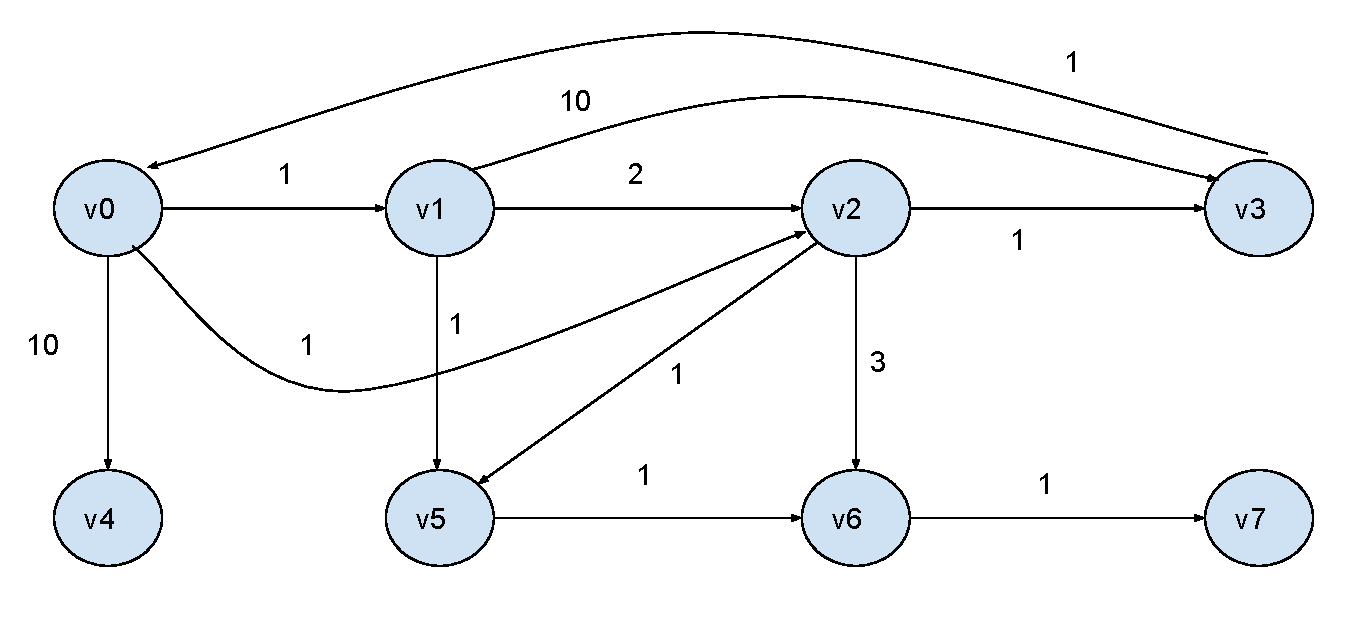
\includegraphics[width=0.9\textwidth]{figures/graph_example.pdf}
\caption{A sample graph}
\label{sssp:example}
\end{figure}

\begin{table}
  \begin{tabular}{| c | }
    \hline
    vid \\ \hline
    0 \\ \hline
    1 \\ \hline
    2 \\ \hline
    3 \\ \hline
    4 \\ \hline
    5 \\ \hline
    6 \\ \hline
    7 \\
    \hline
  \end{tabular}
  \quad
  \begin{tabular}{| c | c | c |}
    \hline
    src & dest & weight \\ \hline
    0 & 1 & 1 \\ \hline
    0 & 2 & 1 \\ \hline
    0 & 4 & 10 \\ \hline
    1 & 2 & 2 \\ \hline
    1 & 3 & 10 \\ \hline
    1 & 5 & 1 \\ \hline
    2 & 3 & 1 \\ \hline
    2 & 5 & 1 \\ \hline
    2 & 6 & 3 \\ \hline
    3 & 0 & 1 \\ \hline
    5 & 6 & 1 \\ \hline
    6 & 7 & 1 \\
    \hline
  \end{tabular}
  \caption{Graph representation of vertices (left) and edges(right) in the
  database}
  \label{sssp:rep}
\end{table}


\section{Single Source Shortest Path} \label{sec:graph:sssp}

Given a graph and a source vertex, single source shortest path (SSSP)
algorithm finds a path for every vertex such that the sum of the weights of
its constituent edges is minimized.

Shortest path is defined as follows. Let $e_{i,j}$ be the edge from vertex $i$
to vertex $j$ and $w_{i,j}$ be its weight. Given a graph G, the shortest path
from $s$ to $d$ is $P = (v_1, v_2 \dots, v_n)$ (where $v_1=s$ and $v_n=d$)
that over all possible $n$ minimizes the sum $ \sum _{i=1}^{n-1}f(e_{i,i+1})$.

% \subsection{Bellman Ford Algorithm}

Bellman-Ford Algorithm \cite{bellman1958routing,ford1956network} is based on
the following idea: We start with a naive approximation for the cost of
reaching every vertex. At each iteration, these values are refined based on
the edge list and the existing approximations. If there are no refinements at
any given step, the algorithm returns the calculated results. If the algorithm
does not converge in $|V|-1$ iterations, this indicates the existence of a
negative cycle in the graph.


\begin{algorithm}[SSSP$(V,E,start)$] \label{alg:sssp}
\alginput{Vertex set $v$, edge set $E$, starting vertex $start$}
\algoutput{Distance and parent set for every vertex $cur$}
\begin{algorithmic}[1]
	\State $toupdate(0) \set (start,0,start)$
	\For{every $i \in 0\dots|V|-1$}
		\For{every tuple $t \in toupdate(i)$} \label{alg:sssp:update}
			\For{every edge $e \mid e.src = t.id$}
		 		\State $local \set e.val + t.val$
		 		\If{$local < toupdate(i+1,e.dest).val$} \label{alg:sssp:single}
		 			\State $toupdate(i+1,dest) \set (local,e.src)$
		 		\EndIf
			\EndFor
		\EndFor
		\For{every tuple $t \in toupdate(i+1)$}
		 	\If{$t.val < cur(t.id).val$}
		 		\State $cur(t.id) \set (t.val,t.parent)$
		 	\EndIf
		\EndFor
	\EndFor
\end{algorithmic}
\end{algorithm}

\begin{description}
\item edge: $(src,dest,val)$. The edges of the graph.
\item cur: $id \rightarrow (val,parent)$. The intermediate SSSP results.
\item toupdate: $iter \rightarrow (id \rightarrow (val,parent))$. The set of updates.
\end{description}

Changes from the standard Bellman-Ford algorithm:

\begin{description}
\item Line~\ref{alg:sssp:update}: We only check the vertices that have been
updated in the last iteration.
\item Line~\ref{alg:sssp:single}: At each iteration, we update a given vertex
only one time. This means the toupdate set cannot contain multiple records
for the same vertex which requires the comparison with the existing value.
\end{description}

This is not a 1-to-1 pseudocode for the implementation since we don't compare
the `toupdate` table records one by one but calculate the overall minimum. In
addition, the comparison with `cur` values take place earlier to reduce the
number of tuples in the `toupdate` table.

\subsection{Implementation Details}

In this section, we discuss the MADlib implementation of the SSSP algorithm
in depth.

\begin{algorithm}[SSSP$(V,E,start)$] \label{alg:sssp:high}
\begin{algorithmic}[1]
	\Repeat
		\State Find Updates
		\State Apply updates to the output table
	\Until {There are no updates}
\end{algorithmic}
\end{algorithm}

The implementation consists of two SQL blocks that are called sequentially
inside a loop. We will follow the example graph at Figure~\ref{sssp:example}
with the starting point as $v_0$. The very first update on the output table is
the source vertex. Its weight is $0$ and its parent is itself ($v_0$). After
this initialization step, the loop starts with Find Updates (the individual
updates will be represented with <dest,value,parent> format). Looking at the
example, it is clear that the updates should be <1,1,0>, <2,1,0> and <4,10,0>.
We will assume this iteration is already completed and look how the next
iteration of the algorithm works to explain the implementation details.

\begin{algorithm}[Find Updates$(E,old\_update,out\_table)$]
\label{alg:sssp:findu}
\begin{lstlisting}
INSERT INTO new_update
	SELECT DISTINCT ON (y.id) y.id AS id,
		y.val AS val,
		y.parent AS parent
	FROM out_table INNER JOIN (
			SELECT edge_table.dest AS id, x.val AS val, old_update.id AS parent
			FROM old_update
				INNER JOIN edge_table
				ON (edge_table.src = old_update.id)
				INNER JOIN (
					SELECT edge_table.dest AS id,
						min(old_update.val + edge_table.weight) AS val
					FROM old_update INNER JOIN
						edge_table AS edge_table ON
						(edge_table.src=old_update.id)
					GROUP BY edge_table.dest
				) x
				ON (edge_table.dest = x.id)
			WHERE ABS(old_update.val + edge_table.weight - x.val) < EPSILON
		) AS y ON (y.id = out_table.vertex_id)
	WHERE y.val<out_table.weight
\end{lstlisting}
\end{algorithm}

The Find Updates query is constructed in 4 levels of subqueries: \emph{find
values, find parents, eliminate duplicates and ensure improvement}.

\begin{itemize}

\item We begin our analysis at the innermost subquery, emph{find values}
(lines 11-16). This subquery takes a set of vertices (in the table
$old\_update$) and finds the reachable vertices. In case a vertex is reachable
by multiple vertices, only the path that has the minimum cost is considered
(hence the name find values). There are two important points to note:
	\begin{itemize}
	\item The input vertices need the value of their path as well.
		\begin{itemize}
		\item In our example, both $v_1$ and $v_2$ can reach $v_3$. We would
		have to use $v_2 \rightarrow v_3$ edge since that gives the lowest possible
		path value.
		\end{itemize}
	\item The subquery is aggregating the rows using the $min$ operator for
	each destination vertex and  unable to return the source vertex at the
	same time to use as the parent value.
		\begin{itemize}
		\item We know the value of $v_3$ should be $2$ but we cannot know
		its parent ($v_2$) at the same time.
		\end{itemize}
	\end{itemize}

\item The \emph{find parents} subquery is designed to solve the
aforementioned limitation. We combine the result of \emph{find values} with
$edge$ and $old\_update$ tables (lines 7-10) and get the rows that has the
same minimum value.
	\begin{itemize}
	\item Note that, we would have to tackle the problem of tie-breaking.
		\begin{itemize}
		\item Vertex $v_5$ has two paths leading into: <5,2,1> and <5,2,2>.
		The inner subquery will return <5,2> and it will match both of these
		edges.
		\end{itemize}
	\item It is redundant to keep both of them in the update list as that
	would require updating the same vertex multiple times in a given
	iteration.
	\end{itemize}

\item At this level, we employ the \emph{eliminate duplicates} subquery. By
using the $DISTINCT$ clause at line 2, we allow the underlying system to
accept only a single one of them.

\item Finally, we introduce the \emph{ensure improvement} subquery to make
sure these updates are actually leading us to shortest paths. Line 21 ensures
that the values stored in the $out\_table$ does not increase and the solution
does not regress throughout the iterations.
\end{itemize}

Applying updates is straightforward as the values and the associated parent
values are replaced using the $new\_update$ table. After this operation is
completed the $new\_update$ table becomes $old\_update$ for the next iteration
of the algorithm.

Please note that, for ideal performance, \emph{vertex} and \emph{edge} tables
should be distributed on \emph{vertex id} and \emph{source id} respectively.

\section{All Pairs Shortest Paths} \label{sec:graph:apsp}

Given a graph and a source vertex, all pairs shortest paths (APSP) algorithm
finds a path for every vertex pair such that the sum of the weights of its
constituent edges is minimized. Please refer to the
Section~\ref{sec:graph:sssp} on single source shortest path for the
mathematical definition of shortest path.

Our implementation has a dynamic programming approach, based on the matrix
multiplication inspired APSP algorithm \cite{apsp}. The idea is similar to
the one from SSSP implementation. We start with a naive approximation for the
cost of every vertex pair (infinite). At each iteration, these values are
refined based on the edge list and the existing approximations. This
refinement step is similar to a matrix multiplication. For every vertex pair
$i,j$, we check every edge $e: j \rightarrow k$ to see if it is possible to
use $e$ to reduce the cost of path $i \rightarrow k$. If there are no
refinements at any given step, the algorithm returns the calculated results.
If the algorithm does not converge in $|V|-1$ iterations, this indicates the
existence of a negative cycle in the graph.

\begin{algorithm}[APSP$(V,E)$] \label{alg:apsp}
\alginput{Vertex set $v$, edge set $E$}
\algoutput{Distance and parent set for every vertex pair}
\begin{algorithmic}[1]

	\While {$update$ is $True$}
		\State $update \set False$
		\For{every vertex pair $i,j$}
			\For{every edge $j \rightarrow k$}
		 		\If{$ val(i \rightarrow j) + val(j \rightarrow k) < val(i \rightarrow k)$}
		 			\State $val(i \rightarrow k) \set  val(i \rightarrow j) + val(j \rightarrow k)$
		 			\State $parent(i \rightarrow k) \set j$
		 			\State $update \set True$
		 		\EndIf
			\EndFor
		\EndFor
	\EndWhile
\end{algorithmic}
\end{algorithm}

\subsection{Implementation Details}

The implementation details are similar to the SSSP as the requirements and
restrictions such as finding the parent, distinct updates, etc. are common in
both cases. This section will mostly focus on the differences in the APSP
implementation.

\begin{algorithm}[Find Updates$(E,out)$]
\label{alg:apsp:findu}
\begin{lstlisting}
INSERT INTO update
	SELECT DISTINCT ON (y.src, y.dest) y.src AS src, y.dest AS dest
		y.val AS val,
		y.parent AS parent
	FROM out INNER JOIN (
			SELECT
				x.src AS src, x.dest AS dest,
				x.val AS val, out.dest AS parent
			FROM out
				INNER JOIN edge_table
				ON (edge_table.src = out.dest)
				INNER JOIN (
					SELECT out.src AS src, edge_table.dest AS dest,
						min(out.val + edge_table.weight) AS val
					FROM out INNER JOIN
						edge_table ON
						(edge_table.src=out.dest)
					GROUP BY out.src, edge_table.dest
				) x
				ON (edge_table.src = x.src AND edge_table.dest = x.dest)
			WHERE ABS(out.val + edge_table.weight - x.val) < EPSILON
		) AS y ON (y.src = out.src AND y.dest = out.dest)
	WHERE y.val < out.val
\end{lstlisting}
\end{algorithm}

The only major difference comes in the innermost subquery (lines 13-18). The
\emph{group by} clause ensures that we try to reduce the weight for every
$out.src$ ($i$) and $edge\_table.dest$ ($k$) pair. The \emph{inner join on}
clause ensures that there is a connecting edge ($j\rightarrow k$) that can be
used for the $i,j$ pair. The rest of the changes are mostly trivial as the
algorithm needs to check for both source and destination during joins (instead
of just the destination).


\section{PageRank} \label{sec:graph:pagerank}
\begin{figure}[h]
    \centering
    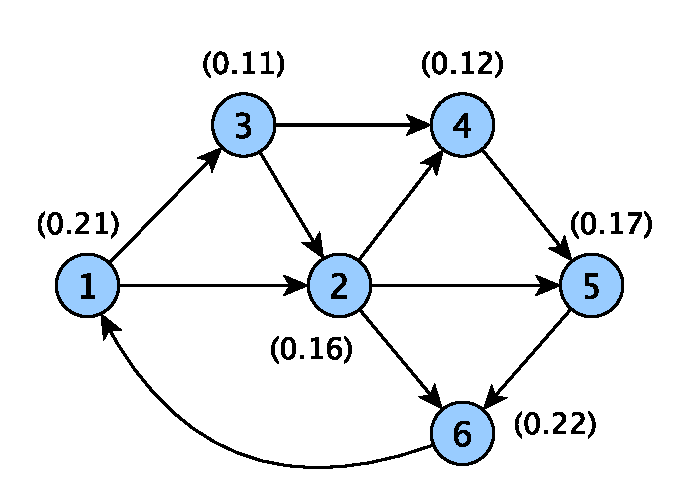
\includegraphics[width=0.5\textwidth]{figures/pagerank_example.pdf}
\caption{An example graph for PageRank}
\label{pagerank:example}
\end{figure}

PageRank is a link analysis algorithm that assigns a score to every vertex
measuring the relative importance of vertices within the set of all
vertices. PageRank~\cite{pagerank} was first used by Google to measure the
importance of website pages where the World Wide Web was modeled as a directed
graph. Figure~\ref{pagerank:example} shows an example graph with the PageRank
value of each vertex. The intuition behind the algorithm is that the number and
quality of links to a vertex determine the authoritativeness of the vertex,
which is reflected in the PageRank scores as shown in the figure.

The pagerank module in MADlib implements the model of a random surfer who
follows the edges of a graph to traverse it, and jumps to a random vertex
after several clicks. The random surfer is modeled using a damping factor
that represents the probability with which the surfer will continue to follow
links in the graph rather than jumping to a random vertex. MADlib's pagerank
module outputs a probability distribution that represents the likelihood that
the random surfer arrives at a particular vertex in the graph.

PageRank is an iterative algorithm where the PageRank scores of vertices from
the previous iteration are used to compute the new PageRank scores. The
PageRank score of a vertex $v$, at the $i^{th}$ iteration, denoted by $PR(v_i)$
is computed as:

\begin{equation}
PR(v_i) = \frac{1-d}{N} + d \sum_{u \in M(v)}(\frac{PR(u_{i-1})}{L(u)})
\label{eq:pagerank}
\end{equation}

where $N$ is the number of vertices in the graph, $d$ is the damping factor,
$M(v)$ represents the set of vertices that have an edge to vertex $v$,
$L(u)$ represents the out-degree of vertex $u$, i.e., the number of
out-going edges from vertex $u$, and $PR(u_{i-1})$ represents the PageRank
score of vertex $u$ in the $(i-1)^{st}$ iteration.

$\frac{1-d}{N}$ represents the tiny probability with which the surfer
would randomly jump to vertex $v$, rather than arriving at $v$ following
links in the graph. This ensures that there is some probability of visiting
every vertex in the graph even if they do not have any incoming edges. Note
that the PageRank score computed for a vertex $v$ using~\ref{eq:pagerank}
in the $i^{th}$ iteration is not updated until the new score is computed for
all the vertices in the graph. The computation terminates either when the
PageRank score of no vertex changes beyond a threshold across two consecutive
iterations, or when a pre-set number of iterations are completed.

\subsection{Implementation Details} \label{sec:pagerank:implementation}

In this section, we discuss the MADlib implementation of PageRank in depth.
We maintain two tables at every iteration: $previous$ and $cur$. The
$previous$ table maintains the PageRank scores of all vertices computed in
the previous iteration, while $cur$ maintains the updated scores of all
vertices in the current iteration.

\begin{algorithm}[PageRank$(V,E)$] \label{alg:pagerank:high}
\begin{algorithmic}[1]
    \State Create $previous$ table with a default PageRank score of
            $\frac{1}{N}$ for every vertex
    \Repeat
        \State Create empty table $cur$.
        \State Update $cur$ using PageRank scores of vertices in $previous$
        \State Update PageRank scores of vertices without incoming edges
        \State Drop $previous$ and rename $cur$ to $previous$
    \Until {PageRank scores have converged or \emph{max} iterations have elapsed}
\end{algorithmic}
\end{algorithm}

The implementation consists of updating the PageRank scores of all vertices
at every iteration, using the PageRank scores of vertices from the previous
iteration. The PageRank score of every vertex is initialized to $\frac{1}{N}$
where $N$ is the total number of vertices in the graph. The out-degree of
every vertex in the graph (represented by $L(u)$ in eq.~\ref{eq:pagerank}),
is captured in table $out\_cnts$. The following query is used to create and
update the PageRank scores in $cur$ table using the PageRank scores in
$previous$ table.

\begin{algorithm}[Update PageRank scores$(previous,out\_cnts,d,N)$]
\label{alg:pagerank:update}
\begin{lstlisting}
CREATE TABLE cur AS
    SELECT edge_table.dest AS id,
        SUM(previous1.pagerank/out_cnts.cnt)*d + (1-d)/N AS pagerank
    FROM edge_table
        INNER JOIN previous ON edge_table.dest = previous.id
        INNER JOIN out_cnts ON edge_table.src = out_cnts.id
        INNER JOIN previous AS previous1 ON edge_table.src = previous1.id
    GROUP BY edge_table.dest

-- Update PageRank scores of vertices without any incoming edges:
INSERT INTO cur
    SELECT id, (1-d)/N AS pagerank
    FROM previous
    WHERE id NOT IN (
        SELECT id
        FROM cur
    )
\end{lstlisting}
\end{algorithm}

The PageRank computation is terminated either when a fixed number of iterations
are completed, or when the PageRank scores of all vertices have converged. The
PageRank score of a vertex is deemed converged if the absolute difference in
its PageRank scores from $previous$ and $cur$ is less than a specified threshold.
The following query is used to find all the vertices whose PageRank scores have
not converged yet.

\begin{algorithm}[Update PageRank scores$(previous,cur,threshold)$]
\label{alg:pagerank:update}
\begin{lstlisting}
SELECT id
FROM cur
INNER JOIN previous ON cur.id = previous.id
WHERE ABS(previous.pagerank - cur.pagerank) > threshold
\end{lstlisting}
\end{algorithm}

\subsection{Best Practices} \label{sec:pagerank:bestpractices}

The pagerank module in MADlib has a few optional parameters: damping factor
$d$, number of iterations $max$, and the threshold for convergence $threshold$.
The default values for these parameters when not specified by the user are
$0.85$, $100$ and $\frac{1}{N*1000}$ respectively.

The damping factor denotes the probability with which the surfer uses the edges
to traverse the graph. If set to $0$, it implies that the only way a surfer
would visit a vertex in the graph is by randomly jumping to it. If set to
$1$, it implies that the only way the surfer can reach a vertex is by following
the edges in the graph, thus precluding the surfer from reaching a vertex
that has no incoming edges. It is common practice to set damping factor
to $0.85$~\cite{pagerank}, and the maximum number of iterations to $100$.
The convergence test for PageRank in MADlib checks for the delta between
the PageRank scores of a vertex across two consecutive iterations. Since
the initial value of the PageRank score is set to $\frac{1}{N}$, the delta
will be small in the initial iterations when $N$ is large (say over 100
million). We thus set the threshold to $\frac{1}{N*1000}$, and it is to be
noted that this is not based on any experimental study. Users of MADlib are
encouraged to consider this factor when setting a value for threshold, since
a high $threshold$ value would lead to early termination of PageRank
computation, thus resulting in incorrect PageRank values.


\section{Weakly Connected Components} \label{sec:graph:wcc}
\begin{figure}[h]
    \centering
    \includegraphics[width=0.5\textwidth]{figures/wcc_example.pdf}
\caption{An example disconnected directed graph}
\label{wcc:example}
\end{figure}

Given a directed graph $G$, a weakly connected component is a subgraph
$G_{sub}$ of $G$, such that there exists a path from every vertex in $G_{sub}$
to every other vertex in $G_{sub}$, ignoring the direction of the edges.

The weakly connected component module implemented in MADlib is based on
GRAIL~\cite{grail}. All vertices are initialized with their own vertex
ID as the component ID, and are considered to be active. In every iteration,
each active vertex's component ID is updated with the smallest component ID
value of all its neighbors. Any vertex whose component ID is not updated in
the current iteration is deemed as an inactive vertex for the next iteration.
Execution continues until there are no active vertices left. Since each vertex
is initialized with its own ID as the component ID, and updated based on
neighboring nodes' component IDs, the final component ID of a component will
be equal to the smallest vertex ID in the corresponding subgraph.
Figure~\ref{wcc:example} shows an example directed graph with two disconnected
subgraphs. The subgraph containing vertices $1$, $2$, $3$, $4$, $5$ and $6$
forms a weakly connected component, and is assigned component ID 1, while the
subgraph containing vertices $12$, $14$, $21$ and $23$ forms the second component
and is assigned component ID 12.

\subsection{Implementation Details} \label{sec:wcc:implementation}

In this section, we discuss the MADlib implementation of weakly connected
components in depth. We maintain the following tables at every iteration:
$oldupdate$, $message$ and $newupdate$. In $newupdate$, the component ID
of each vertex is initialized to infinity, while the component ID of vertices
in the $message$ table is initialized to their corresponding vertex ID.

\begin{algorithm}[Weakly Connected Components$(V,E)$] \label{alg:wcc:high}
\begin{algorithmic}[1]
    \State Create $newupdate$ table with a default component ID of
            $infinity$ for every vertex
    \State Create $message$ table with a default component ID of the
            corresponding $id$ (vertex ID) for every vertex
    \Repeat
        \State Update the $oldupdate$ table
        \State Update $toupdate$ table with active vertices
        \State Update the $newupdate$ table
        \State Update $message$ table with potential new component IDs for each vertex
    \Until {There are no active vertices in $toupdate$ table}
\end{algorithmic}
\end{algorithm}

The $message$ table contains the component IDs associated with all its
immediate neighbors. At each iteration, $oldupdate$ is updated with the
minimum of all the associated component IDs found for a vertex in $message$.

\begin{algorithm}[Update oldupdate table]
\begin{lstlisting}
SELECT id, MIN(message.component_id) as component_id
FROM message
GROUP BY id
\end{lstlisting}
\end{algorithm}

Table $toupdate$ records all vertices whose component IDs must be updated,
and are thus marked active.

\begin{algorithm}[Update toupdate table with active vertices]
\begin{lstlisting}
-- Find vertices whose component ID must be updated
CREATE TABLE toupdate AS
SELECT id, component_id
FROM oldupdate, newupdate
WHERE oldupdate.id = newupdate.id AND
        oldupdate.component_id < newupdate.component_id

-- Update the component IDs
UPDATE newupdate SET
component_id = toupdate.component_id
FROM toupdate
WHERE newupdate.id = toupdate.id
\end{lstlisting}
\end{algorithm}

Finally, the $message$ table is updated with potential new
component IDs for active vertices using the following query:

\begin{algorithm}[Update oldupdate table]
\begin{lstlisting}
CREATE TEMP TABLE message AS
SELECT id, MIN(component_id) AS component_id
FROM (
    SELECT edge.src AS id,
        toupdate.component_id
    FROM toupdate, edge
    WHERE edge.dest = toupdate.id
    UNION ALL
    SELECT edge.dest AS id,
        toupdate.component_id
    FROM toupdate, edge
    WHERE edge.src = toupdate.id
) AS t
GROUP BY id
\end{lstlisting}
\end{algorithm}

At the end of the computation, $newupdate$ will have the component ID
associated with each vertex in $G$. The component ID of all the vertices
in a component is equal to the smallest vertex ID in the corresponding
subgraph.

\section{Breadth-first Search} \label{sec:graph:bfs}

Given a graph $G$ and a user-specified origin vertex $src$, this algorithm
searches and discovers connected nodes in a graph in breadth-first order
\cite{bfs_wikipedia}. The graph can be treated as either directed or
undirected based on a parameter specified when calling the function.
There is also a parameter to control the number of hops (edges) to traverse
from the source vertex. If not specified, all nodes accessible from the
source node will be discovered.

\subsection{Implementation Details}
\begin{algorithm}[Breadth First Search$(V, E, src)$] \label{alg:bfs:high}
\begin{algorithmic}[1]
    \State Set $dist \leftarrow 0$
    \State Create $message$ table with $src$ vertex, $NULL$ parent, and $dist$
    \State Copy $message$ table to output table $out$
    \Repeat
        \State Create $toupdate$ table using $out$ and $message$ tables
        \State $dist \leftarrow dist + 1$
        \State Update $message$ table with newly found candidate vertices, parent and $dist$
        \State Copy $message$ table to $out$
    \Until {There are no candidate vertices remaining in $message$ table}
\end{algorithmic}
\end{algorithm}

The implementation details are similar to SSSP, albeit simpler. We only have to
track the number of hops and not the sum of weights, but other requirements and
restrictions such as finding the parent, distinct updates, etc. are common in
both cases. The output table is initialized only to the $src$ vertex to begin
with. A $message$ table is also maintained that contains the list of vertices
to traverse and explore in the next iteration, which is also initialized with
the $src$ vertex. BFS then runs iteratively until no more candidate vertices
remain in the $message$ table, as outlined in~\ref{alg:bfs:high}.

At every iteration, $toupdate$ table is updated with vertices that are neighbors
of vertices in the $message$ table, that are not already visited in the past
(one scan of the $out$ table reveals all the vertices that have already been
visited in the past). All such newly found neighboring vertices in the current
iteration will have one or more parents, based on how many vertices in the
$message$ table have a direct edge to them. Each such vertex in the $message$
table is marked as the parent of such newly found neighboring vertices in
the $toupdate$ table.

The $message$ table is then cleared and updated with the contents of $toupdate$
table, except that for each new neighboring vertex considered, only one of the
parents is recorded as its parent (the node with the smallest id among all
parent nodes). The content of this updated $message$ is then copied
to the $out$ table, and this process continues until $message$ table is empty.

% Licensed to the Apache Software Foundation (ASF) under one
% or more contributor license agreements.  See the NOTICE file
% distributed with this work for additional information
% regarding copyright ownership.  The ASF licenses this file
% to you under the Apache License, Version 2.0 (the
% "License"); you may not use this file except in compliance
% with the License.  You may obtain a copy of the License at

%   http://www.apache.org/licenses/LICENSE-2.0

% Unless required by applicable law or agreed to in writing,
% software distributed under the License is distributed on an
% "AS IS" BASIS, WITHOUT WARRANTIES OR CONDITIONS OF ANY
% KIND, either express or implied.  See the License for the
% specific language governing permissions and limitations
% under the License.

% When using TeXShop on the Mac, let it know the root document.
% The following must be one of the first 20 lines.
% !TEX root = ../design.tex

\chapter{Neural Network}

\begin{moduleinfo}
\item[Authors] {Xixuan Feng, Cooper Sloan}
\end{moduleinfo}

% Abstract. What is the problem we want to solve?
This module implements artificial neural network \cite{ann_wiki}.

\section{Multilayer Perceptron}
Multilayer perceptron is arguably the most popular model among many neural network models \cite{mlp_wiki}.
Here, we learn the coefficients by minimizing a least square objective function, or cross entropy (\cite{bertsekas1999nonlinear}, example 1.5.3).
The parallel architecture is based on the paper by Zhiheng Huang \cite{mlp_parallel}.

% Background. Why can we solve the problem with gradient-based methods?
\subsection{Solving as a Convex Program}
Although the objective function is not necessarily convex, gradient descent or incremental gradient descent are still commonly-used algorithms to learn the coefficients.
To clarify, gradient-based methods are not different from the famous backpropagation, which is essentially a way to compute the gradient value.

\subsection{Formal Description}
Having the convex programming framework, the main tasks of implementing a learner include:
(a) choose a subset of algorithms;
(b) implement the related computation logic for the objective function, e.g., gradient.

For multilayer perceptron, we choose incremental gradient descent (IGD).
In the remaining part of this section, we will give a formal description of the derivation of objective function and its gradient.

\paragraph{Objective function.}
We mostly follow the notations in example 1.5.3 from Bertsekas \cite{bertsekas1999nonlinear}, for a multilayer perceptron that has $N$ layers (stages), and the $k^{th}$ stage has $n_k$ activation units ($\phi : \mathbb{R} \to \mathbb{R}$), the objective function for regression is given as
\[f_{(x, y)}(u) = \frac{1}{2} \|h(u, x) - y\|_2^2,\]
and for classification the objective function is given as
\[f_{(x, y)}(u) = \sum_i (\log(h_i(u, x)) * z_i + (1-\log(h_i(u, x))) *( 1- z_i) ,\]
where $x \in \mathbb{R}^{n_0}$ is the input vector, $y \in \mathbb{R}^{n_N}$ is the output vector (one hot encoded for classification),~\footnote{Of course, the objective function can be defined over a set of input-output vector pairs, which is simply given as the addition of the above $f$.}
and the coefficients are given as
\[u = \{ u_{k-1}^{sj} \; | \; k = 1,...,N, \: s = 0,...,n_{k-1}, \: j = 1,...,n_k\},\]
And are initialized from a uniform distribution as follows:
\[u_{k}^{sj} = uniform(-r,r),\]
where r is defined as follows:
\[r = \sqrt{\frac{6}{n_k+n_{k+1}}}\]
With regularization, an additional term enters the objective function, given as
\[\sum_{u_k^{sj}} \frac{1}{2} \lambda u_k^{sj2} \]
This still leaves $h : \mathbb{R}^{n_0} \to \mathbb{R}^{n_N}$ as an open item.
Let $o_k \in \mathbb{R}^{n_k}, k = 1,...,N$ be the output vector of the $k^{th}$ layer. Then we define $h(u, x) = o_N$, based on setting $o_0 = x$ and the $j^{th}$ component of $o_k$ is given in an iterative fashion as~\footnote{$o_k^0 \equiv 1$ is used to simplified the notations, and $o_k^0$ is not a component of $o_k$, for any $k = 0,...,N$.}
\[\begin{alignedat}{5}
    o_k^j = \phi \left( \sum_{s=0}^{n_{k-1}} o_{k-1}^s u_{k-1}^{sj} \right), &\quad k = 1,...,N, \; j = 1,...,n_k
\end{alignedat}\]

\paragraph{Gradient of the End Layer.}
Let's first handle $u_{N-1}^{st}, s = 0,...,n_{N-1}, t = 1,...,n_N$.
Let $y^t$ denote the $t^{th}$ component of $y \in \mathbb{R}^{n_N}$, and $h^t$ the $t^{th}$ component of output of $h$.
\[\begin{aligned}
    \frac{\partial f}{\partial u_{N-1}^{st}}
    &= \left( h^t(u, x) - y^t \right) \cdot \frac{\partial h^t(u, x)}{\partial u_{N-1}^{st}} \\
    &= \left( o_N^t - y^t \right) \cdot \frac{\partial o_N^t}{\partial u_{N-1}^{st}} \\
    &= \left( o_N^t - y^t \right) \cdot \frac{\partial \phi \left( \sum_{s=0}^{n_{N-1}} o_{N-1}^s u_{N-1}^{st} \right)}{\partial u_{N-1}^{st}} \\
    &= \left( o_N^t - y^t \right) \cdot \phi' \left( \sum_{s=0}^{n_{N-1}} o_{N-1}^s u_{N-1}^{st} \right) \cdot o_{N-1}^s \\
\end{aligned}\]
To ease the notation, let the input vector of the $j^{th}$ activation unit of the $(k+1)^{th}$ layer be
\[\mathit{net}_k^j =\sum_{s=0}^{n_{k-1}} o_{k-1}^s u_{k-1}^{sj},\]
where $k = 1,...,N, \; j = 1,...,n_k$, and note that $o_k^j =\phi(\mathit{net}_k^j)$. Finally, the gradient
\[\frac{\partial f}{\partial u_{N-1}^{st}} = \left( o_N^t - y^t \right) \cdot \phi' ( \mathit{net}_N^t ) \cdot o_{N-1}^s\]
For any $s = 0,...,n_{N-1}, t =1,...,n_N$, we are given $y^t$, and $o_N^t, \mathit{net}_N^t, o_{N-1}^s$ can be computed by forward iterating the network layer by layer (also called the feed-forward pass). Therefore, we now know how to compute the coefficients for the end layer $u_{N-1}^{st}, s = 0,...,n_{N-1}, t =1,...,n_N$.

\subsubsection{Backpropagation}
For inner (hidden) layers, it is more difficult to compute the partial derivative over the input of activation units (i.e., $\mathit{net}_k, k = 1,...,N-1$).
That said, $\frac{\partial f}{\partial \mathit{net}_N^t} = (o_N^t - y^t) \phi'(\mathit{net}_N^t)$ is easy, where $t = 1,...,n_N$, but $\frac{\partial f}{\partial \mathit{net}_k^j}$ is hard, where $k = 1,...,N-1, j = 1,..,n_k$.
This hard-to-compute statistic is referred to as \textit{delta error}, and let $\delta_k^j = \frac{\partial f}{\partial \mathit{net}_k^j}$, where $k = 1,...,N-1, j = 1,..,n_k$.
If this is solved, the gradient can be easily computed as follow
\[\frac{\partial f}{\partial u_{k-1}^{sj}} = \boxed{\frac{\partial f}{\partial \mathit{net}_k^j}} \cdot \frac{\partial \mathit{net}_k^j}{\partial u_{k-1}^{sj}} = \boxed{\delta_k^j} o_{k-1}^s,\]
where $k = 1,...,N-1, s = 0,...,n_{k-1}, j = 1,..,n_k$.
To solve this, we introduce the popular backpropagation below.

\paragraph{Error Back Propagation.}
Since we know how to compute $\delta_N^t, t = 1,...,n_N$, we try to compute $\delta_{k}^j, j = 1,...,n_{k}$, given $\delta_{k+1}^t, t = 1,...,n_{k+1}$, for any $k = 1,...,N-1$.
First,
\[
    \delta_{k}^j
    = \frac{\partial f}{\partial \mathit{net}_{k}^j}
    = \frac{\partial f}{\partial o_{k}^j} \cdot \frac{\partial o_{k}^j}{\partial \mathit{net}_{k}^j}
    = \frac{\partial f}{\partial o_{k}^j} \cdot \phi'(\mathit{net}_{k}^j)
\]

\[\begin{alignedat}{5}
    \frac{\partial f}{\partial o_{k}^j} = \sum_{t=1}^{n_{k+1}} \left( \frac{\partial f}{\partial \mathit{net}_{k+1}^t} \cdot \frac{\partial \mathit{net}_{k+1}^t}{\partial o_{k}^j} \right),
    &\quad k = 1,...,N-1, \: j = 1,...,n_{k}
\end{alignedat}\]
Using the above equation, we can solve delta error backward iteratively
\[\begin{aligned}
    \delta_{k}^j
    &= \frac{\partial f}{\partial o_{k}^j} \cdot \phi'(\mathit{net}_{k}^j) \\
    &= \sum_{t=1}^{n_{k+1}} \left( \frac{\partial f}{\partial \mathit{net}_{k+1}^t} \cdot \frac{\partial \mathit{net}_{k+1}^t}{\partial o_{k}^j} \right) \cdot \phi'(\mathit{net}_{k}^j) \\
    &= \sum_{t=1}^{n_{k+1}} \left( \delta_{k+1}^t \cdot \frac{\partial \left( \sum_{s=0}^{n_{k}} o_{k}^s u_{k}^{st} \right) }{\partial o_{k}^j} \right) \cdot \phi'(\mathit{net}_{k}^j) \\
    &= \sum_{t=1}^{n_{k+1}} \left( \delta_{k+1}^t \cdot u_{k}^{jt} \right) \cdot \phi'(\mathit{net}_{k}^j) \\
\end{aligned}\]
To sum up, we need the following equation for error back propagation
\[\boxed{\delta_{k}^j = \sum_{t=1}^{n_{k+1}} \left( \delta_{k+1}^t \cdot u_{k}^{jt} \right) \cdot \phi'(\mathit{net}_{k}^j)}\]
where $k = 1,...,N-1$, and $j = 1,...,n_{k}$.

\subsubsection{The $\mathit{Gradient}$ Function}
\begin{algorithm}[mlp-gradient$(u, x, y)$] \label{alg:mlp-gradient}
\alginput{Coefficients $u = \{ u_{k-1}^{sj} \; | \; k = 1,...,N, \: s = 0,...,n_{k-1}, \: j = 1,...,n_k\}$,\\
start vector $x \in \mathbb{R}^{n_0}$,\\
end vector $y \in \mathbb{R}^{n_N}$,\\
activation unit $\phi : \mathbb{R} \to \mathbb{R}$}
\algoutput{Gradient value $\nabla f(u)$ that consists of components $\nabla f(u)_{k-1}^{sj} = \frac{\partial f}{\partial u_{k-1}^{sj}}$}
\begin{algorithmic}[1]
    \State $(\mathit{net}, o) \set$ \texttt{feed-forward}$(u, x, \phi)$
    \State $\delta_N \set$ \texttt{end-layer-delta-error}$(\mathit{net}, o, y, \phi')$
    \State $\delta \set$ \texttt{back-propogate}$(\mathit{net}, o, y, u, \phi')$
    \For{$k = 1,...,N$}
        \For{$s = 0,...,n_{k-1}$}
            \For{$j = 1,...,n_k$}
                \State $\nabla f(u)_{k-1}^{sj} \set \delta_k^j o_{k-1}^s$
                \Comment{Can be put together with the computation of delta $\delta$}
            \EndFor
        \EndFor
    \EndFor
    \State \Return $\nabla f(u)$
\end{algorithmic}
\end{algorithm}

\paragraph{Activation Units $\phi$.}
Common examples of activation units are
\[\begin{alignedat}{3}
\phi(\xi) &= \frac{1}{1 + e^{-\xi}}, &\quad \text{ (logistic function),}\\
\phi(\xi) &= \frac{e^{\xi} - e^{-\xi}}{e^{\xi} + e^{-\xi}}, &\quad \text{ (hyperbolic tangent function)}\\
\phi(\xi) &= max(x,0), &\quad \text{ (rectified linear function)}\\
\end{alignedat}\]

\begin{algorithm}[feed-forward$(u, x, \phi)$] \label{alg:feed-forward}
\alginput{Coefficients $u = \{ u_{k-1}^{sj} \; | \; k = 1,...,N, \: s = 0,...,n_{k-1}, \: j = 1,...,n_k\}$,\\
input vector $x \in \mathbb{R}^{n_0}$,\\
activation unit $\phi : \mathbb{R} \to \mathbb{R}$}
\algoutput{Input vectors $\mathit{net} = \{\mathit{net}_k^j \; | \; k = 1,...,N, \: j = 1,...,n_k\}$,\\
output vectors $o = \{o_k^j \; | \; k = 0,...,N, \: j = 0,...,n_k\}$}
\begin{algorithmic}[1]
    \For{$k = 0,...,N$}
        \State $o_k^0 \set 1$
    \EndFor
    \State $o_0 \set x$ \Comment{For all components $o_0^j, x^j, \; j = 1,...,n_0$}
    \For{$k = 1,...,N$}
        \For{$j = 1,...,n_k$}
            \State $\mathit{net}_k^j \set 0$
            \For{$s = 0,...,n_{k-1}$}
                \State $\mathit{net}_k^j \set \mathit{net}_k^j + o_{k-1}^s u_{k-1}^{sj}$
            \EndFor
            \State $o_k^j = \phi(\mathit{net}_k^j)$ \Comment{Where the activation function for the final layer is identity for regression and softmax for classification.}
        \EndFor
    \EndFor
    \State \Return $(\mathit{net}, o)$
\end{algorithmic}
\end{algorithm}

\begin{algorithm}[back-propogate$(\delta_N, \mathit{net}, u, \phi')$] \label{alg:back-propogate}
\alginput{input vectors $\mathit{net} = \{\mathit{net}_k^j \; | \; k = 1,...,N, \: j = 1,...,n_k\}$,\\
output vectors $o = \{o_k^j \; | \; k = 0,...,N, \: j = 0,...,n_k\}$,\\
end vector $y \in \mathbb{R}^{n_N}$,\\
coefficients $u = \{ u_{k-1}^{sj} \; | \; k = 1,...,N, \: s = 0,...,n_{k-1}, \: j = 1,...,n_k\}$,\\
derivative of activation unit $\phi' : \mathbb{R} \to \mathbb{R}$}
\algoutput{Delta $\delta = \{\delta_k^j \; | \; k = 1,...,N, \: j = 1,...,n_k\}$}
\begin{algorithmic}[1]
    \For{$t = 1,...,n_N$}
            \State $\delta_N^t \set (o_N^t - y^t)$ \Comment{This applies for identity activation and mean square error loss and softmax activation with cross entropy loss}
    \EndFor
    \For{$k = N-1,...,1$}
        \For{$j = 0,...,n_k$}
            \State $\delta_k^j \set 0$
            \For{$t = 1,...,n_{k+1}$}
                \State $\delta_k^j \set \delta_k^j + \delta_{k+1}^t u_k^{jt}$
            \EndFor
            \State $\delta_k^j \set \delta_k^j \phi'(\mathit{net}_k^j)$
        \EndFor
    \EndFor
    \State \Return $\delta$
\end{algorithmic}
\end{algorithm}

\begin{algorithm}[mlp-train-iteration$(X, Y, \eta)$] \label{alg:mlp-train-iteration}
\alginput{
start vectors $X_{i...m} \in \mathbb{R}^{n_0}$,\\
end vectors $Y_{i...m} \in \mathbb{R}^{n_N}$,\\
learning rate $\eta$,\\}
\algoutput{Coefficients $u = \{ u_{k-1}^{sj} \; | \; k = 1,...,N, \: s = 0,...,n_{k-1}, \: j = 1,...,n_k\}$}
\begin{algorithmic}[1]
    \State \texttt{Randomnly initialize u}
    \For{$i = 1,...,m$}
        \State $\nabla f(u) \set \texttt{mlp-gradient}(u,X_i,Y_i)$
        \State $u \set u - (\eta \nabla f(u) u + \lambda u)$
    \EndFor
    \State \Return $u$
\end{algorithmic}
\end{algorithm}

\begin{algorithm}[mlp-train-parallel$(X, Y, \eta, s, t)$] \label{alg:mlp-train-parallel}
\alginput{
start vectors $X_{i...m} \in \mathbb{R}^{n_0}$,\\
end vectors $Y_{i...m} \in \mathbb{R}^{n_N}$,\\
learning rate $\eta$,\\
segments $s$,\\
iterations $t$,\\}
\algoutput{Coefficients $u = \{ u_{k-1}^{sj} \; | \; k = 1,...,N, \: s = 0,...,n_{k-1}, \: j = 1,...,n_k\}$}
\begin{algorithmic}[1]
    \State \texttt{Randomnly initialize u}
    \For{$j = 1,...,s$}
        \State $X_j \set \texttt{subset-of-X}$
        \State $Y_j \set \texttt{subset-of-Y}$
    \EndFor
    \For{$i = 1,...,t$}
        \For{$j = 1,...,s$}
            \State $u_j \set copy(u)$
            \State $u_j \set \texttt{mlp-train-iteration}(X_j, Y_j, \eta)$
        \EndFor
        \State $u \set \texttt{weighted-avg}(u_{1...s})$
    \EndFor
    \State \Return $u$
\end{algorithmic}
\end{algorithm}

% Licensed to the Apache Software Foundation (ASF) under one
% or more contributor license agreements.  See the NOTICE file
% distributed with this work for additional information
% regarding copyright ownership.  The ASF licenses this file
% to you under the Apache License, Version 2.0 (the
% "License"); you may not use this file except in compliance
% with the License.  You may obtain a copy of the License at

%   http://www.apache.org/licenses/LICENSE-2.0

% Unless required by applicable law or agreed to in writing,
% software distributed under the License is distributed on an
% "AS IS" BASIS, WITHOUT WARRANTIES OR CONDITIONS OF ANY
% KIND, either express or implied.  See the License for the
% specific language governing permissions and limitations
% under the License.

!TEX root = ../design.tex


\chapter[k Nearest Neighbors]{k Nearest Neighbors}

\begin{moduleinfo}
\item[Authors] \href{mailto:okislal@pivotal.io}{Orhan Kislal}

\item[History]
	\begin{modulehistory}
		\item[v0.1] Initial version: knn and kd-tree.
	\end{modulehistory}
\end{moduleinfo}


% Abstract. What is the problem we want to solve?
\section{Introduction} % (fold)
\label{sec:knn_introduction}

\emph{Some notes and figures in this section are borrowed from \cite{medium_knn} and \cite{point_knn}}.

K-nearest neighbors (KNN) is one of the most commonly used learning
algorithms. The goal of knn is to find a number (k) of training data points
closest to the test point. These neighbors can be used to predict labels via
classification or regression.

KNN does not have a training phase like the most of learning techniques. It
does not create a model to generalize the data, instead the algorithm uses the
whole training dataset (or a specific subset of it).

KNN can be used for classification, the output is a class membership (a
discrete value). An object is classified by a majority vote of its neighbors,
with the object being assigned to the class most common among its k nearest
neighbors. It can also be used for regression, output is the value for the
object (predicts continuous values). This value is the average (or median) of
the values of its k nearest neighbors.

\section{Implementation Details}

The basic KNN implementation depends on the table join between the training dataset and the test dataset.

\begin{sql}
	(SELECT test_id,
            train_id,
            fn_dist(train_col_name, test_col_name) AS dist,
            label
    FROM train_table, test_table) AS knn_sub
\end{sql}

Once we have the distance between every train - test pair, the algorithm picks the k smallest values.

\begin{sql}
	SELECT row_number() OVER
        (PARTITION BY test_id ORDER BY dist) AS r,
        test_id,
        train_id,
        label
	FROM knn_sub
	WHERE r <= k
\end{sql}

Finally, the prediction is completed based on the labels of the selected
training points for each test point.

\section{Enabling KD-tree}

One of the major shortcomings of KNN is the fact that it is computationally
expensive. In addition, there is no training phase; which means every single
prediction will have to compute the full table join. One of the ways to
improve the performance is to reduce the search space for test points. Kd-tree
option is developed to enable trading the accuracy of the output with higher
performance by reducing the neighbor search space.

Kd-trees are used for organizing data in k dimensions. It is constructed like
a binary search tree where each level of the tree is using a specific
dimension for finding splits.


\begin{figure}[h]
	\centering
	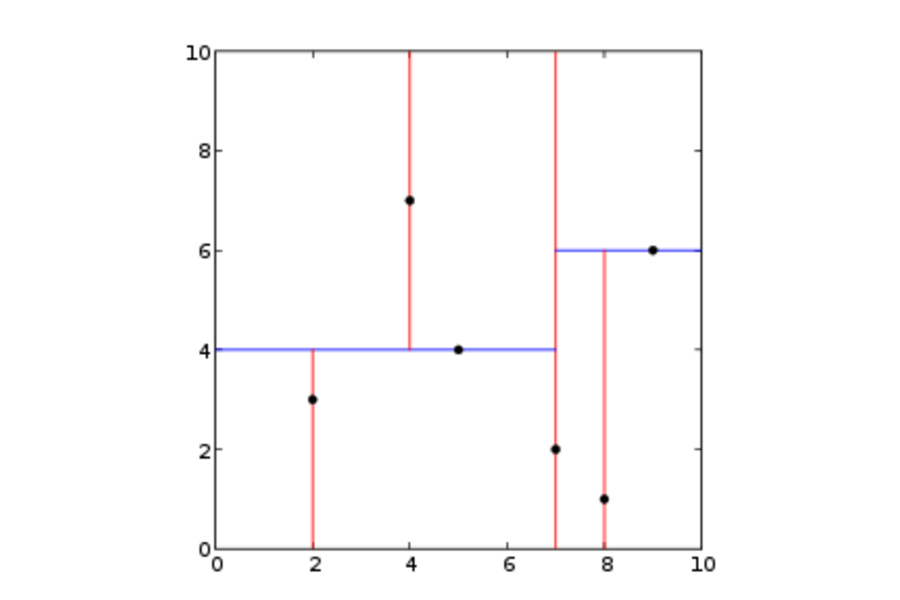
\includegraphics[width=0.9\textwidth]{figures/2d_kdtree.pdf}
\caption{A 2D kd-tree of depth 3}
\label{kdd:2d_kdtree}
\end{figure}

A kd-tree is constructed by finding the median value of the data in a
particular dimension and separating the data into two sections based on this
value. This process is repeated a number of times to construct smaller
regions. Once the kd-tree is prepared, it can be used by any test point to
find its assigned region and this fragmentation can be used for limiting the
search space for nearest neighbors.

Once we have the kd-tree regions and their borders, we find the associated
regions for the test points. This gives us the first region to search for
nearest neighbors. In addition, we allow the user to request for multiple
regions to search. This means we have to decide which additional regions to
include in our search. We implemented a backtracking algorithm to find these
regions. The core idea is to find the closest border for each test point and
select the region on the other side of the border. Note that points that
reside in the same region might have different secondary (or tertiary, etc.)
regions. Consider the tree at Figure~\ref{kdd:2d_kdtree}. A test point at $<5
, 2>$ is in the same region as $<3 , 3.9>$. However, their closest borders and
the associated secondary regions are wildly different. In addition, consider
$<3 , 3.9>$ and $<6 , 3.9>$. They both have the same border as their closest
one ($y=4$). However, their closest regions do differ. To make sure that we
get the correct region, the following scheme is implemented. For a given point
$P$, we find the closest border, $dim[i] = x$ and $P$'s relative position to
it ($pos$ = $-1$ for lower and $+1$ for higher). We conjure a new point that
consists of the same values as the test point in every dimension except $i$.
For $dim[i]$, we set the value to $x-pos*\epsilon$. Finally, we use the
existing kd-tree to find this new point's assigned region. This region is our
expansion target for the point $P$. We repeat this process with the next
closest border as requested by the user.

The knn algorithm does not change significantly with the addition of regions.
Assuming that the training and test datasets have their region information
stored in the tables, the only necessary change is ensuring that the table
join uses these region ids to limit the search space.


\begin{sql}
	(SELECT test_id,
            train_id,
            fn_dist(train_col_name, test_col_name) AS dist,
            label
    FROM train_table, test_table
    WHERE train_table.region_id = test_table.region_id
    ) AS knn_sub
\end{sql}

\printbibliography

\end{document}
